% REV00 Tue 04 May 2021 13:55:16 WIB
% START Tue 04 May 2021 13:55:16 WIB

\chapter{XXX}

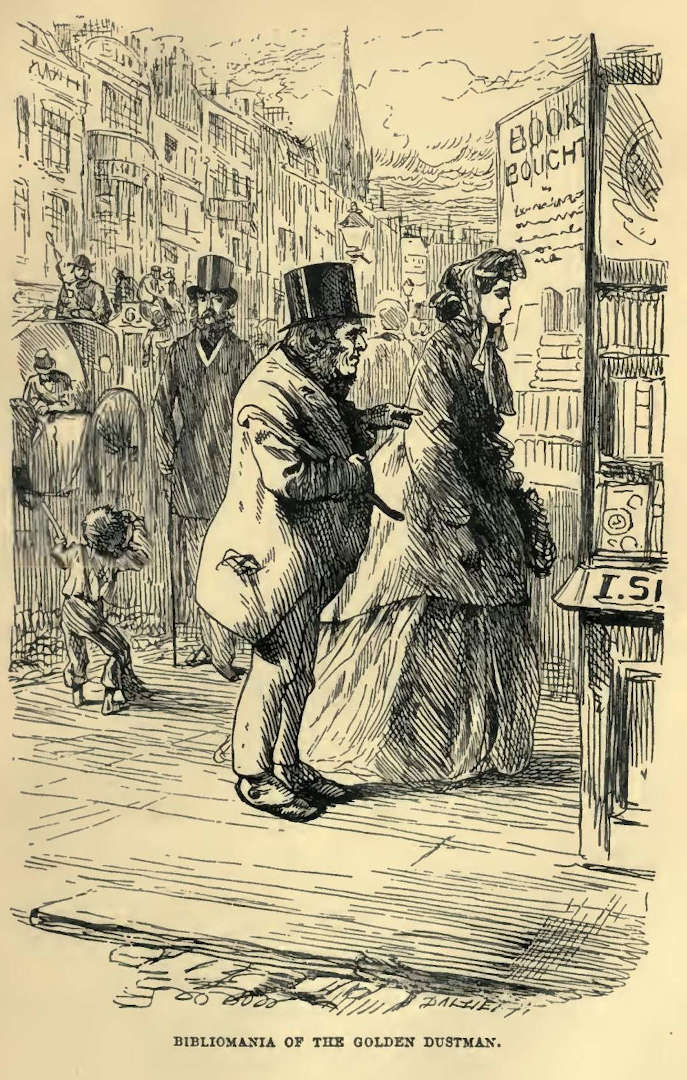
\includegraphics[scale=2.3]{03-05-01}

Chapter 13

GIVE A DOG A BAD NAME, AND HANG HIM


Fascination Fledgeby, left alone in the counting-house, strolled about
with his hat on one side, whistling, and investigating the drawers, and
prying here and there for any small evidences of his being cheated,
but could find none. ‘Not his merit that he don’t cheat me,’ was Mr
Fledgeby’s commentary delivered with a wink, ‘but my precaution.’ He
then with a lazy grandeur asserted his rights as lord of Pubsey and
Co. by poking his cane at the stools and boxes, and spitting in the
fireplace, and so loitered royally to the window and looked out into the
narrow street, with his small eyes just peering over the top of Pubsey
and Co.’s blind. As a blind in more senses than one, it reminded him
that he was alone in the counting-house with the front door open. He was
moving away to shut it, lest he should be injudiciously identified with
the establishment, when he was stopped by some one coming to the door.

This some one was the dolls’ dressmaker, with a little basket on her
arm, and her crutch stick in her hand. Her keen eyes had espied Mr
Fledgeby before Mr Fledgeby had espied her, and he was paralysed in his
purpose of shutting her out, not so much by her approaching the door, as
by her favouring him with a shower of nods, the instant he saw her. This
advantage she improved by hobbling up the steps with such despatch that
before Mr Fledgeby could take measures for her finding nobody at home,
she was face to face with him in the counting-house.

‘Hope I see you well, sir,’ said Miss Wren. ‘Mr Riah in?’

Fledgeby had dropped into a chair, in the attitude of one waiting
wearily. ‘I suppose he will be back soon,’ he replied; ‘he has cut
out and left me expecting him back, in an odd way. Haven’t I seen you
before?’

‘Once before--if you had your eyesight,’ replied Miss Wren; the
conditional clause in an under-tone.

‘When you were carrying on some games up at the top of the house. I
remember. How’s your friend?’

‘I have more friends than one, sir, I hope,’ replied Miss Wren. ‘Which
friend?’

‘Never mind,’ said Mr Fledgeby, shutting up one eye, ‘any of your
friends, all your friends. Are they pretty tolerable?’

Somewhat confounded, Miss Wren parried the pleasantry, and sat down in a
corner behind the door, with her basket in her lap. By-and-by, she said,
breaking a long and patient silence:

‘I beg your pardon, sir, but I am used to find Mr Riah at this time, and
so I generally come at this time. I only want to buy my poor little two
shillings’ worth of waste. Perhaps you’ll kindly let me have it, and
I’ll trot off to my work.’

‘I let you have it?’ said Fledgeby, turning his head towards her; for he
had been sitting blinking at the light, and feeling his cheek. ‘Why, you
don’t really suppose that I have anything to do with the place, or the
business; do you?’

‘Suppose?’ exclaimed Miss Wren. ‘He said, that day, you were the
master!’

‘The old cock in black said? Riah said? Why, he’d say anything.’

‘Well; but you said so too,’ returned Miss Wren. ‘Or at least you took
on like the master, and didn’t contradict him.’

‘One of his dodges,’ said Mr Fledgeby, with a cool and contemptuous
shrug. ‘He’s made of dodges. He said to me, “Come up to the top of the
house, sir, and I’ll show you a handsome girl. But I shall call you
the master.” So I went up to the top of the house and he showed me the
handsome girl (very well worth looking at she was), and I was called the
master. I don’t know why. I dare say he don’t. He loves a dodge for
its own sake; being,’ added Mr Fledgeby, after casting about for an
expressive phrase, ‘the dodgerest of all the dodgers.’

‘Oh my head!’ cried the dolls’ dressmaker, holding it with both her
hands, as if it were cracking. ‘You can’t mean what you say.’

‘I can, my little woman, retorted Fledgeby, ‘and I do, I assure you.’

This repudiation was not only an act of deliberate policy on Fledgeby’s
part, in case of his being surprised by any other caller, but was also a
retort upon Miss Wren for her over-sharpness, and a pleasant instance
of his humour as regarded the old Jew. ‘He has got a bad name as an old
Jew, and he is paid for the use of it, and I’ll have my money’s worth
out of him.’ This was Fledgeby’s habitual reflection in the way of
business, and it was sharpened just now by the old man’s presuming
to have a secret from him: though of the secret itself, as annoying
somebody else whom he disliked, he by no means disapproved.

Miss Wren with a fallen countenance sat behind the door looking
thoughtfully at the ground, and the long and patient silence had
again set in for some time, when the expression of Mr Fledgeby’s face
betokened that through the upper portion of the door, which was of
glass, he saw some one faltering on the brink of the counting-house.
Presently there was a rustle and a tap, and then some more rustling and
another tap. Fledgeby taking no notice, the door was at length softly
opened, and the dried face of a mild little elderly gentleman looked in.

‘Mr Riah?’ said this visitor, very politely.

‘I am waiting for him, sir,’ returned Mr Fledgeby. ‘He went out and left
me here. I expect him back every minute. Perhaps you had better take a
chair.’

The gentleman took a chair, and put his hand to his forehead, as if
he were in a melancholy frame of mind. Mr Fledgeby eyed him aside, and
seemed to relish his attitude.

‘A fine day, sir,’ remarked Fledgeby.

The little dried gentleman was so occupied with his own depressed
reflections that he did not notice the remark until the sound of Mr
Fledgeby’s voice had died out of the counting-house. Then he started,
and said: ‘I beg your pardon, sir. I fear you spoke to me?’

‘I said,’ remarked Fledgeby, a little louder than before, ‘it was a fine
day.’

‘I beg your pardon. I beg your pardon. Yes.’

Again the little dried gentleman put his hand to his forehead, and again
Mr Fledgeby seemed to enjoy his doing it. When the gentleman changed his
attitude with a sigh, Fledgeby spake with a grin.

‘Mr Twemlow, I think?’

The dried gentleman seemed much surprised.

‘Had the pleasure of dining with you at Lammle’s,’ said Fledgeby. ‘Even
have the honour of being a connexion of yours. An unexpected sort of
place this to meet in; but one never knows, when one gets into the City,
what people one may knock up against. I hope you have your health, and
are enjoying yourself.’

There might have been a touch of impertinence in the last words; on the
other hand, it might have been but the native grace of Mr Fledgeby’s
manner. Mr Fledgeby sat on a stool with a foot on the rail of another
stool, and his hat on. Mr Twemlow had uncovered on looking in at the
door, and remained so. Now the conscientious Twemlow, knowing what he
had done to thwart the gracious Fledgeby, was particularly disconcerted
by this encounter. He was as ill at ease as a gentleman well could be.
He felt himself bound to conduct himself stiffly towards Fledgeby,
and he made him a distant bow. Fledgeby made his small eyes smaller
in taking special note of his manner. The dolls’ dressmaker sat in her
corner behind the door, with her eyes on the ground and her hands folded
on her basket, holding her crutch-stick between them, and appearing to
take no heed of anything.

‘He’s a long time,’ muttered Mr Fledgeby, looking at his watch. ‘What
time may you make it, Mr Twemlow?’

Mr Twemlow made it ten minutes past twelve, sir.

‘As near as a toucher,’ assented Fledgeby. ‘I hope, Mr Twemlow, your
business here may be of a more agreeable character than mine.’

‘Thank you, sir,’ said Mr Twemlow.

Fledgeby again made his small eyes smaller, as he glanced with great
complacency at Twemlow, who was timorously tapping the table with a
folded letter.

‘What I know of Mr Riah,’ said Fledgeby, with a very disparaging
utterance of his name, ‘leads me to believe that this is about the shop
for disagreeable business. I have always found him the bitingest and
tightest screw in London.’

Mr Twemlow acknowledged the remark with a little distant bow. It
evidently made him nervous.

‘So much so,’ pursued Fledgeby, ‘that if it wasn’t to be true to a
friend, nobody should catch me waiting here a single minute. But if you
have friends in adversity, stand by them. That’s what I say and act up
to.’

The equitable Twemlow felt that this sentiment, irrespective of the
utterer, demanded his cordial assent. ‘You are very right, sir,’ he
rejoined with spirit. ‘You indicate the generous and manly course.’

‘Glad to have your approbation,’ returned Fledgeby. ‘It’s a coincidence,
Mr Twemlow;’ here he descended from his perch, and sauntered towards
him; ‘that the friends I am standing by to-day are the friends at whose
house I met you! The Lammles. She’s a very taking and agreeable woman?’

Conscience smote the gentle Twemlow pale. ‘Yes,’ he said. ‘She is.’

‘And when she appealed to me this morning, to come and try what I could
do to pacify their creditor, this Mr Riah--that I certainly have gained
some little influence with in transacting business for another friend,
but nothing like so much as she supposes--and when a woman like that
spoke to me as her dearest Mr Fledgeby, and shed tears--why what could I
do, you know?’

Twemlow gasped ‘Nothing but come.’

‘Nothing but come. And so I came. But why,’ said Fledgeby, putting
his hands in his pockets and counterfeiting deep meditation, ‘why Riah
should have started up, when I told him that the Lammles entreated him
to hold over a Bill of Sale he has on all their effects; and why he
should have cut out, saying he would be back directly; and why he should
have left me here alone so long; I cannot understand.’

The chivalrous Twemlow, Knight of the Simple Heart, was not in a
condition to offer any suggestion. He was too penitent, too remorseful.
For the first time in his life he had done an underhanded action, and he
had done wrong. He had secretly interposed against this confiding young
man, for no better real reason than because the young man’s ways were
not his ways.

But, the confiding young man proceeded to heap coals of fire on his
sensitive head.

‘I beg your pardon, Mr Twemlow; you see I am acquainted with the nature
of the affairs that are transacted here. Is there anything I can do for
you here? You have always been brought up as a gentleman, and never as a
man of business;’ another touch of possible impertinence in this place;
‘and perhaps you are but a poor man of business. What else is to be
expected!’

‘I am even a poorer man of business than I am a man, sir,’ returned
Twemlow, ‘and I could hardly express my deficiency in a stronger way. I
really do not so much as clearly understand my position in the matter
on which I am brought here. But there are reasons which make me
very delicate of accepting your assistance. I am greatly, greatly,
disinclined to profit by it. I don’t deserve it.’

Good childish creature! Condemned to a passage through the world by such
narrow little dimly-lighted ways, and picking up so few specks or spots
on the road!

‘Perhaps,’ said Fledgeby, ‘you may be a little proud of entering on the
topic,--having been brought up as a gentleman.’

‘It’s not that, sir,’ returned Twemlow, ‘it’s not that. I hope I
distinguish between true pride and false pride.’

‘I have no pride at all, myself,’ said Fledgeby, ‘and perhaps I don’t
cut things so fine as to know one from t’other. But I know this is a
place where even a man of business needs his wits about him; and if mine
can be of any use to you here, you’re welcome to them.’

‘You are very good,’ said Twemlow, faltering. ‘But I am most
unwilling--’

‘I don’t, you know,’ proceeded Fledgeby with an ill-favoured glance,
‘entertain the vanity of supposing that my wits could be of any use
to you in society, but they might be here. You cultivate society and
society cultivates you, but Mr Riah’s not society. In society, Mr Riah
is kept dark; eh, Mr Twemlow?’

Twemlow, much disturbed, and with his hand fluttering about his
forehead, replied: ‘Quite true.’

The confiding young man besought him to state his case. The innocent
Twemlow, expecting Fledgeby to be astounded by what he should unfold,
and not for an instant conceiving the possibility of its happening every
day, but treating of it as a terrible phenomenon occurring in the course
of ages, related how that he had had a deceased friend, a married civil
officer with a family, who had wanted money for change of place or
change of post, and how he, Twemlow, had ‘given him his name,’ with the
usual, but in the eyes of Twemlow almost incredible result that he had
been left to repay what he had never had. How, in the course of years,
he had reduced the principal by trifling sums, ‘having,’ said Twemlow,
‘always to observe great economy, being in the enjoyment of a fixed
income limited in extent, and that depending on the munificence of
a certain nobleman,’ and had always pinched the full interest out of
himself with punctual pinches. How he had come, in course of time,
to look upon this one only debt of his life as a regular quarterly
drawback, and no worse, when ‘his name’ had some way fallen into the
possession of Mr Riah, who had sent him notice to redeem it by paying up
in full, in one plump sum, or take tremendous consequences. This, with
hazy remembrances of how he had been carried to some office to ‘confess
judgment’ (as he recollected the phrase), and how he had been carried
to another office where his life was assured for somebody not wholly
unconnected with the sherry trade whom he remembered by the remarkable
circumstance that he had a Straduarius violin to dispose of, and also a
Madonna, formed the sum and substance of Mr Twemlow’s narrative. Through
which stalked the shadow of the awful Snigsworth, eyed afar off by
money-lenders as Security in the Mist, and menacing Twemlow with his
baronial truncheon.

To all, Mr Fledgeby listened with the modest gravity becoming a
confiding young man who knew it all beforehand, and, when it was
finished, seriously shook his head. ‘I don’t like, Mr Twemlow,’ said
Fledgeby, ‘I don’t like Riah’s calling in the principal. If he’s
determined to call it in, it must come.’

‘But supposing, sir,’ said Twemlow, downcast, ‘that it can’t come?’

‘Then,’ retorted Fledgeby, ‘you must go, you know.’

‘Where?’ asked Twemlow, faintly.

‘To prison,’ returned Fledgeby. Whereat Mr Twemlow leaned his innocent
head upon his hand, and moaned a little moan of distress and disgrace.

‘However,’ said Fledgeby, appearing to pluck up his spirits, ‘we’ll hope
it’s not so bad as that comes to. If you’ll allow me, I’ll mention to Mr
Riah when he comes in, who you are, and I’ll tell him you’re my friend,
and I’ll say my say for you, instead of your saying it for yourself; I
may be able to do it in a more business-like way. You won’t consider it
a liberty?’

‘I thank you again and again, sir,’ said Twemlow. ‘I am strong,
strongly, disinclined to avail myself of your generosity, though my
helplessness yields. For I cannot but feel that I--to put it in the
mildest form of speech--that I have done nothing to deserve it.’

‘Where CAN he be?’ muttered Fledgeby, referring to his watch again.
‘What CAN he have gone out for? Did you ever see him, Mr Twemlow?’

‘Never.’

‘He is a thorough Jew to look at, but he is a more thorough Jew to deal
with. He’s worst when he’s quiet. If he’s quiet, I shall take it as a
very bad sign. Keep your eye upon him when he comes in, and, if he’s
quiet, don’t be hopeful. Here he is!--He looks quiet.’

With these words, which had the effect of causing the harmless Twemlow
painful agitation, Mr Fledgeby withdrew to his former post, and the old
man entered the counting-house.

‘Why, Mr Riah,’ said Fledgeby, ‘I thought you were lost!’

The old man, glancing at the stranger, stood stock-still. He perceived
that his master was leading up to the orders he was to take, and he
waited to understand them.

‘I really thought,’ repeated Fledgeby slowly, ‘that you were lost, Mr
Riah. Why, now I look at you--but no, you can’t have done it; no, you
can’t have done it!’

Hat in hand, the old man lifted his head, and looked distressfully at
Fledgeby as seeking to know what new moral burden he was to bear.

‘You can’t have rushed out to get the start of everybody else, and put
in that bill of sale at Lammle’s?’ said Fledgeby. ‘Say you haven’t, Mr
Riah.’

‘Sir, I have,’ replied the old man in a low voice.

‘Oh my eye!’ cried Fledgeby. ‘Tut, tut, tut! Dear, dear, dear! Well! I
knew you were a hard customer, Mr Riah, but I never thought you were as
hard as that.’

‘Sir,’ said the old man, with great uneasiness, ‘I do as I am directed.
I am not the principal here. I am but the agent of a superior, and I
have no choice, no power.’

‘Don’t say so,’ retorted Fledgeby, secretly exultant as the old man
stretched out his hands, with a shrinking action of defending himself
against the sharp construction of the two observers. ‘Don’t play the
tune of the trade, Mr Riah. You’ve a right to get in your debts, if
you’re determined to do it, but don’t pretend what every one in your
line regularly pretends. At least, don’t do it to me. Why should you, Mr
Riah? You know I know all about you.’

The old man clasped the skirt of his long coat with his disengaged hand,
and directed a wistful look at Fledgeby.

‘And don’t,’ said Fledgeby, ‘don’t, I entreat you as a favour, Mr Riah,
be so devilish meek, for I know what’ll follow if you are. Look here, Mr
Riah. This gentleman is Mr Twemlow.’

The Jew turned to him and bowed. That poor lamb bowed in return; polite,
and terrified.

‘I have made such a failure,’ proceeded Fledgeby, ‘in trying to do
anything with you for my friend Lammle, that I’ve hardly a hope of doing
anything with you for my friend (and connexion indeed) Mr Twemlow. But
I do think that if you would do a favour for anybody, you would for me,
and I won’t fail for want of trying, and I’ve passed my promise to Mr
Twemlow besides. Now, Mr Riah, here is Mr Twemlow. Always good for his
interest, always coming up to time, always paying his little way. Now,
why should you press Mr Twemlow? You can’t have any spite against Mr
Twemlow! Why not be easy with Mr Twemlow?’

The old man looked into Fledgeby’s little eyes for any sign of leave to
be easy with Mr Twemlow; but there was no sign in them.

‘Mr Twemlow is no connexion of yours, Mr Riah,’ said Fledgeby; ‘you
can’t want to be even with him for having through life gone in for a
gentleman and hung on to his Family. If Mr Twemlow has a contempt for
business, what can it matter to you?’

‘But pardon me,’ interposed the gentle victim, ‘I have not. I should
consider it presumption.’

‘There, Mr Riah!’ said Fledgeby, ‘isn’t that handsomely said? Come! Make
terms with me for Mr Twemlow.’

The old man looked again for any sign of permission to spare the poor
little gentleman. No. Mr Fledgeby meant him to be racked.

‘I am very sorry, Mr Twemlow,’ said Riah. ‘I have my instructions. I am
invested with no authority for diverging from them. The money must be
paid.’

‘In full and slap down, do you mean, Mr Riah?’ asked Fledgeby, to make
things quite explicit.

‘In full, sir, and at once,’ was Riah’s answer.

Mr Fledgeby shook his head deploringly at Twemlow, and mutely expressed
in reference to the venerable figure standing before him with eyes upon
the ground: ‘What a Monster of an Israelite this is!’

‘Mr Riah,’ said Fledgeby.

The old man lifted up his eyes once more to the little eyes in Mr
Fledgeby’s head, with some reviving hope that the sign might be coming
yet.

‘Mr Riah, it’s of no use my holding back the fact. There’s a certain
great party in the background in Mr Twemlow’s case, and you know it.’

‘I know it,’ the old man admitted.

‘Now, I’ll put it as a plain point of business, Mr Riah. Are you fully
determined (as a plain point of business) either to have that said great
party’s security, or that said great party’s money?’

‘Fully determined,’ answered Riah, as he read his master’s face, and
learnt the book.

‘Not at all caring for, and indeed as it seems to me rather enjoying,’
said Fledgeby, with peculiar unction, ‘the precious kick-up and row that
will come off between Mr Twemlow and the said great party?’

This required no answer, and received none. Poor Mr Twemlow, who had
betrayed the keenest mental terrors since his noble kinsman loomed in
the perspective, rose with a sigh to take his departure. ‘I thank you
very much, sir,’ he said, offering Fledgeby his feverish hand. ‘You have
done me an unmerited service. Thank you, thank you!’

‘Don’t mention it,’ answered Fledgeby. ‘It’s a failure so far, but I’ll
stay behind, and take another touch at Mr Riah.’

‘Do not deceive yourself Mr Twemlow,’ said the Jew, then addressing him
directly for the first time. ‘There is no hope for you. You must expect
no leniency here. You must pay in full, and you cannot pay too promptly,
or you will be put to heavy charges. Trust nothing to me, sir. Money,
money, money.’ When he had said these words in an emphatic manner, he
acknowledged Mr Twemlow’s still polite motion of his head, and that
amiable little worthy took his departure in the lowest spirits.

Fascination Fledgeby was in such a merry vein when the counting-house
was cleared of him, that he had nothing for it but to go to the window,
and lean his arms on the frame of the blind, and have his silent laugh
out, with his back to his subordinate. When he turned round again with a
composed countenance, his subordinate still stood in the same place, and
the dolls’ dressmaker sat behind the door with a look of horror.

‘Halloa!’ cried Mr Fledgeby, ‘you’re forgetting this young lady, Mr
Riah, and she has been waiting long enough too. Sell her her waste,
please, and give her good measure if you can make up your mind to do the
liberal thing for once.’

He looked on for a time, as the Jew filled her little basket with such
scraps as she was used to buy; but, his merry vein coming on again, he
was obliged to turn round to the window once more, and lean his arms on
the blind.

‘There, my Cinderella dear,’ said the old man in a whisper, and with a
worn-out look, ‘the basket’s full now. Bless you! And get you gone!’

‘Don’t call me your Cinderella dear,’ returned Miss Wren. ‘O you cruel
godmother!’

She shook that emphatic little forefinger of hers in his face at
parting, as earnestly and reproachfully as she had ever shaken it at her
grim old child at home.

‘You are not the godmother at all!’ said she. ‘You are the Wolf in
the Forest, the wicked Wolf! And if ever my dear Lizzie is sold and
betrayed, I shall know who sold and betrayed her!’



